% !TeX root = ../report.tex
% !TeX spellcheck = en-US
% !TeX encoding = UTF-8
\section{COVERAGE PATH PLANNING}\label{sec:cpp}
Two of the use cases described in the introduction dictate that the crawler has to cover the whole area preferably with
an \gls{gls-optimal-path}. This type of path planning problem differs from the in Chapter~\ref{sec:cpp} described
problem. \citeauthor{choset_principles_2005} describes the task of determining a path that passes an effector (e.g., a
robot, a detector, etc.) over all points in a free space as a~\gls{gls-coverage-path}
problem~\cite{choset_principles_2005}, hence that this task is called a~\gls[first]{acr-CPP}. This type of task can be
found as an integral part of many robotic applications such as vacuum cleaning robots, painter robots, autonomous
underwater vehicles creating image mosaic, demining robots, lawn mowers, automated harvesters, window cleaners and
inspection of complex underwater structures~\cite{galceran_survey_2013}.

All these type of robots need to cover a complete region in order to perform their tasks. According to
\citet{cao_region_1988} such a mobile robot should use the following criteria, for a region filling operation
\begin{enumerate}
	\setlength\itemsep{0mm}
	\item The mobile robot must move through an entire area, i.e., the overall travel must cover a whole region.
	\item The mobile robot must fill the region without overlapping paths.
	\item Continuous and sequential operations without any repetition of paths is required of the robot.
	\item The robot must avoid all obstacles in a region.
	\item Simple motion trajectories (e.g., straight lines or circles) should be used for simplicity in control.
	\item An ``optimal'' path is desired under the available conditions. it's not always possible to satisfy all these
	criteria for a complex environment. Sometimes a priority consideration is required.
\end{enumerate}

\citet{galceran_towards_2014} describes that these types coverage algorithms can be classified as \emph{heuristic} or
\emph{complete} depending on whether or not the provable guarantee complete coverage of the free space. At the same time
they can be classified as \gls{gls-off-line} or \gls{gls-on-line}. \gls{gls-off-line} algorithm rely on only on
stationary information, and the environment is assumed to be known. Usually \gls{gls-on-line} algorithms are needed if
some kind of adaptivity to the requirement is required. On-line algorithms usually utilize real-time sensor
measurements. Thus these algorithms can also be called \emph{sensor-based coverage algorithms}. \gls{gls-on-line}
coverage algorithms are in effect ``\emph{divide and conquer}'' strategies, which \citet{wong_complete_2004} describes
as a powerful technique used to solve many problems and many mapping procedures carry out a process of space
decomposition, where a complex space is repeatedly divided until simple sub-regions of a particular type are created. The
problem at hand is then solved by applying a simpler algorithm to the simpler sub-regions.

Since an autonomous operating crawler can be stationed in different environments with multiple unknown obstacles, the
focus of this chapter lies on \gls{gls-on-line} or sensor-based coverage algorithms from which the following are
identified:
\begin{itemize}
	\item morse-based cellular decomposition
	\begin{itemize}
		\item On-line Morse-based boustrophedon decomposition
		\item Morse-based cellular decomposition combined with generalized \gls{gls-voronoi-diagram}
	\end{itemize}
	\item Landmark-based topological coverage
	\begin{itemize}
		\item Slice decomposition
		\item On-line topological coverage algorithm
	\end{itemize}
	\item Grid-based methods
	\begin{itemize}
		\item Grid-based coverage using spanning trees
		\item Neural network-based coverage on grid maps
	\end{itemize}
	\item Coverage under uncertainty
	\item Multi-robot methods
\end{itemize}

\subsection{MORSE-BASED CELLULAR DECOMPOSITION}
Morse-based cellular decomposition is mostly based upon the following method exact or approximate cellular
decomposition \citet{acar_morse_2002} State that exact cellular decompositions represent the free space
of a robot by dividing it into non-overlapping region sub-level cells such that the union of the cells fills the free
space. Complete coverage is then reduced to ensuring that the robot visits each cell. These cells are constructed using
\gls{gls-morse-function}, a function for which all \gls{gls-critical-point} are non-degenerate and all critical levels
are different.

Morse-functions are visualized by \citet{nicolaescu_invitation_2007} as follows: Suppose \( M \) is a smooth, compact
manifold which is  assumed to be embedded in a Euclidean space \( \Eu \), and from which we would like to understand
some basic topological invariants. This is done with a ``slicing'' technique.

Were a unit vector \gls{sym-u} is fixed in \( \Eu \) and which start slicing \( M \) with the family of hyperplanes
perpendicular to  \gls{sym-u}. Such a hyperplane will in general intersect \( M \) along a submanifold (slice). The
manifold can be recovered by continuously stacking the slices on top of each other in the same order as they were cut
out of \( M \).

If this collection of slices is visualized as a deck of cards with various shapes, which are piled up in the order that
they were produced, there will be an increasing stack of slices. As this stack grows, it can be observed that at certain
moments in time the shape suffers a qualitative change. The theory proposed by Morse extracts quantifiable information,
through studying the evolution of this growing stack of slices.

Each moment in time that this pile changes is called a critical value, which correspond to moments in time when the
hyperplane intersect tangentially. These points marks the boundary of a cell. \citet{acar_morse_2002} states that Morse
theory assures that between those \gls{gls-critical-point} ``merging'' and ``severing'' of slices does not occur and
that a robot can trivially perform simple motions, such as back and forth motions between \gls{gls-critical-point}s and
thus guarantee complete coverage of a cell. Hence this method is duped Morse-based cellular decomposition

The above described method is depicted in figure~\ref{fig:exact_cellular_decomposition} (a). Such an environment can be
represented with a graph such as shown in figure~\ref{fig:exact_cellular_decomposition} (b). Each critical value
corresponds with a node while a cell is represented by an edge.

\begin{RoyalFigure}[!htb, label=fig:exact_cellular_decomposition]{(a) Exact cellular decomposition, (b) Graph representation}
	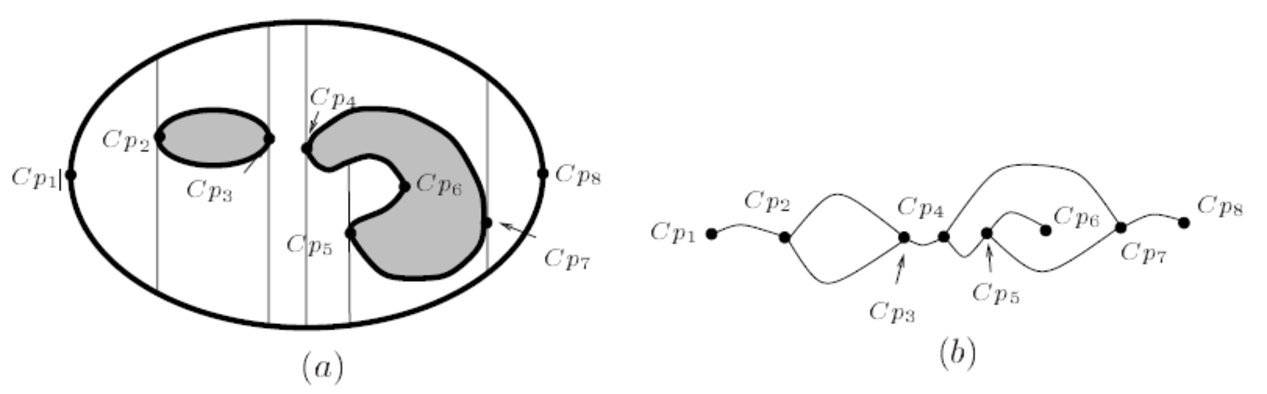
\includegraphics[width=\textwidth,trim=2 2 2 2,clip]{exact_cellular_decomposition.pdf}
\end{RoyalFigure}

The above describe technique has a minor short-coming, \citet{choset_exact_2000} states that this method may result in
many small cell, such as cell 9 shown in figure~\ref{fig:manysmallcells}, which can seemingly be ``clumped'' into
neighbouring cells. Reorganizing the cells can result in a shorter (more efficient) path to cover the same area. To
address this issue, the \gls[first]{acr-BCD} approach was introduced.

\begin{RoyalFigure}[!htb, label=fig:manysmallcells]{TRAPEZOIDAL DECOMPOSITION OF BOUND FREE SPACE\cite{choset_exact_2000}.}
		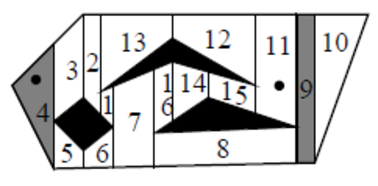
\includegraphics[width=0.4\textwidth,trim=2 2 2 2,clip]{manysmallcells.pdf}
\end{RoyalFigure}

Boustrophedon which literally means ``\emph{the way of the ox}'' merges these cells, such that a more
\gls{gls-optimal-path} can be found. This can be done by using different \gls{gls-morse-function}, which results in
different slice shapes and therefore different cell decompositions, as is shown in
figure~\ref{fig:diffmorsefunction}~\cite{galceran_survey_2013}\cite{choset_coverage_2000}\cite{acar_morse_2002}. Such as
spiral, spike or squarel.

\begin{RoyalFigure}[!htb, label=fig:diffmorsefunction]{SPIRAL, SPIKE AND SQUAREL~\cite{acar_morse_2002}}
		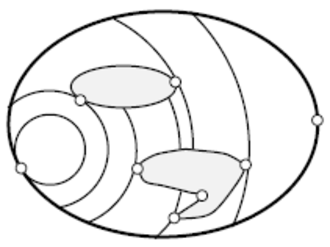
\includegraphics[width=0.3\textwidth,trim=2 2 2 2,clip]{bous1.pdf}
		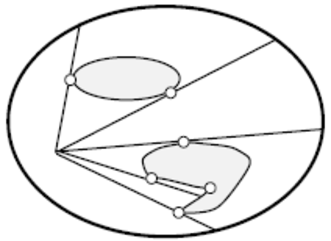
\includegraphics[width=0.3\textwidth,trim=2 2 2 2,clip]{bous2.pdf}
		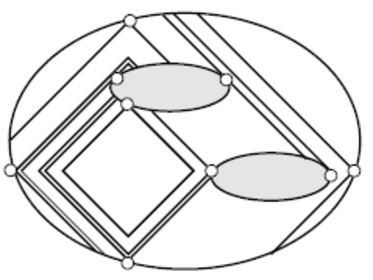
\includegraphics[width=0.3\textwidth,trim=2 2 2 2,clip]{bous3.pdf}
\end{RoyalFigure}

Once each cell is identified a strategy for the infill is executed, which is described by \citet{huang_optimal_2001} as
\gls{gls-coverage-path}s. Each region [or cell red.] is decomposed into sub-regions, a
\gls{gls-traveling-salesman-problem} algorithm, is applied to generate a sequence of sub-regions to visit, and a
\gls{gls-coverage-path} is generated from this sequence that covers each subregion in turn. \citet{huang_optimal_2001}
claims that turns take a significant amount of time: the robot must slow down, make the turn and accelerate. Thus by
minimizing the number of turns, which are proportional to the altitude of a subregion, an \gls{gls-optimal-path} can be
found.

\begin{RoyalFigure}[!htb]{DIFFERENT SWEEP DIRECTIONS~\cite{huang_optimal_2001}}
		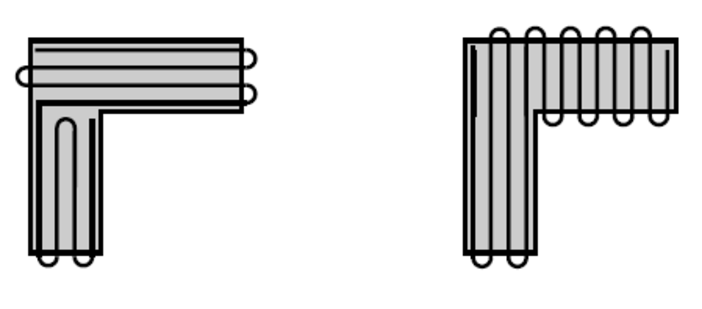
\includegraphics[width=.6\textwidth,trim=2 2 2 2,clip]{differentsweepdirections.pdf}
\end{RoyalFigure}

This is done by first creating an \gls{gls-adjacency-graph} \gls{sym-G_adj}, generated with the
\gls{gls-morse-function}, see figure~\ref{fig:exact_cellular_decomposition} (b). This graph is split in two
\gls{sym-G_adj_1}  and \gls{sym-G_adj_2} sub-graphs. These contain all edges from \gls{sym-G_adj} except those that
connect a node from \gls{sym-G_adj_1} to \gls{sym-G_adj_2}. With this definition the minimum sum of altitudes can be
stated as equation~\ref{eq:MSA}. Where \( i \) iterates over all possibles ways to split graph \gls{sym-G_adj} and \(
\gls{sym-C}(\gls{sym-G_adj} ) \) returns the cost of covering all cells corresponding to nodes in \gls{sym-G_adj}, once
an optimum is found, movements of the sub-regions are implemented.

Let \gls{sym-G_adj_1} and \gls{sym-G_adj_2} be a subset of graph \gls{sym-G_adj} which consist of all the nodes that
needs to be visited and let \gls{sym-C} be a function that calculates the cost in movement \gls{sym-S}, which iterative
over \( i \) for all possible combinations of \gls{sym-G_adj_1} and \gls{sym-G_adj_2}.

\begin{equation}\label{eq:MSA}
	\gls{sym-S}(\gls{sym-G_adj}) = min \left\lbrace \gls{sym-C}(\gls{sym-G_adj}), \underset{i}{min}\  \gls{sym-S} \left(
	\gls{sym-G_adj_1}^i \right) + \gls{sym-S} \left( \gls{sym-G_adj_2}^1 \right) \right\rbrace
\end{equation}

So far it assumed that the environment is known \emph{a priori} which labels this method as an \gls{gls-off-line}
method. While the use case described in Chapter~\ref{chap:introduction}, dictates that the crawler encounters unknown
obstacles.

\subsubsection{ON-LINE MORSE-BASED BOUSTROPHEDON DECOMPOSITION}\label{subsec:onlinemorsebased}
 \citet{acar_sensor_based_2002} describe a method which allows the use of above portrayed Morse-based cellular
 decomposition in an unknown dynamically chancing environment. Critical point sensing, is a way to determine
 \gls{gls-critical-point}s based on a sweep direction and an omnidirectional range sensor. These can be  detected when
 the sweep direction and the surface normal \( \gls{sym-nabla_m}(x) \) of an obstacle are parallel.

\begin{RoyalFigure}[!htb, label=fig:incrementalsweep]{INCREMENTAL GRAPH CONSTRUCTION~\cite{acar_sensor_based_2002}}
	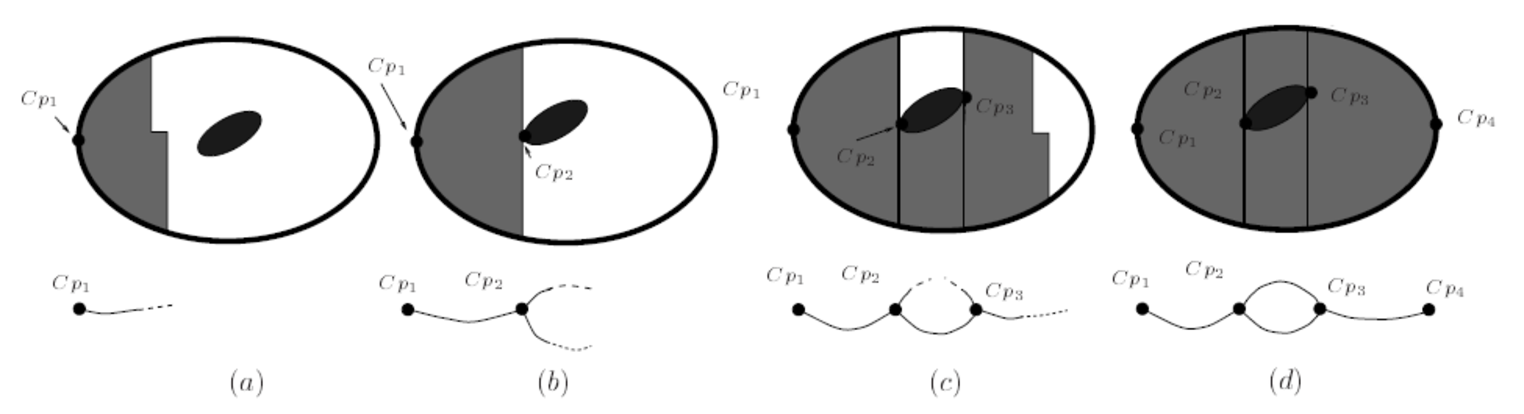
\includegraphics[width=\textwidth,trim=2 2 2 2,clip]{incrementalsweep.pdf}
\end{RoyalFigure}

On-line region coverage is depicted in figure~\ref{fig:incrementalsweep} which shows an incremental sweep as part of an
on-line \gls{acr-BCD} (a) The robot starts to cover the space at the \gls{gls-critical-point} \gls{sym-Cp_1} and
instantiates an edge in the graph. (b) When the robot is done covering the cell between \gls{sym-Cp_1} and
\gls{sym-Cp_2}, it joins the nodes in the graph that correspond to \gls{sym-Cp_1} and \gls{sym-Cp_2} with an edge, and
start two new edges. (c) The robot covers the cells below the obstacle and to the right of \gls{sym-Cp_3}. (d) While
covering the cell above the obstacle, the robot encounters \gls{sym-Cp_2} again. Since all the \gls{gls-critical-point}
have explored edges, i.e., covered cells, the robot concludes that it has completely covered the space
\cite{acar_sensor_based_2002}.

On-line detection of \gls{gls-critical-point}s is illustrated by \citet{galceran_survey_2013}. They tell how a robot
detects a surface normal which is the same as a gradient. Given a robot located at point \gls{sym-x}, let \gls{sym-Cp_0}
be the closest point to \gls{sym-x}  on the surface of obstacle \gls{sym-Cp_i}:

\begin{equation}\label{eq:closestpoint}
	\gls{sym-Cp_0}  = \underset{\gls{sym-x}  \in \gls{sym-Cp_i} }{arg min} ||\gls{sym-x} - \gls{sym-Cp} ||,
\end{equation}

\noindent and let \gls{sym-d_x_i} be the distance between point \gls{sym-x} and the obstacle \gls{sym-Cp_i}. Now, the
gradient of \( \gls{sym-d_x_i}, \nabla \gls{sym-d_x_i} \) can be calculated as

\begin{equation}\label{eq:gradiantdix}
	\nabla \gls{sym-d_x_i} = \frac{\gls{sym-x}  - \gls{sym-Cp_0}}{||\gls{sym-x}  - \gls{sym-Cp_0}||}.
\end{equation}

Since a gradient is a unit vector normal to a surface at a given point and since \gls{sym-Cp_0} is a point laying on the
surface \gls{sym-Cp_i}, \( \gls{sym-x} - \gls{sym-Cp_0} \) is a vector pointing outwards, from \gls{sym-Cp_0} to
\gls{sym-x}, by dividing it by its norm  \( ||\gls{sym-x} - \gls{sym-Cp_0}|| \) it becomes a unit vector. This leads to
the conclusion that a \gls{gls-critical-point} occurs when \( \nabla \gls{sym-d_x_i} \) is parallel to the sweep
direction, as illustrated in figure~\ref{fig:criticalpointdetectiononline}.

\begin{RoyalFigure}[!htb, label=fig:criticalpointdetectiononline]{CRITICAL POINT DETECTING~\cite{galceran_survey_2013}}
		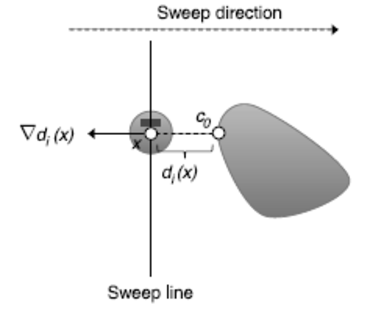
\includegraphics[width=.4\textwidth,trim=2 2 2 2,clip]{critcialpointdetection.pdf}
\end{RoyalFigure}

Points are only detected from the side view. A normal sweeping motion will miss \gls{gls-critical-point} that lay
parallel to the sweep direction. This can be counteracted with a Cyclic path. It's important to note that such a path
will be longer then a normal zig-zag sweep, since it includes backtracking. A cyclic path starts forward

Cyclic path start by moving the robot in a forward phase, when it hits the boundary, it begins moves downwards. When an
obstacles is encounter during its travels it changes it state into a wall following unit, until reaching the next
boundary in front of him or detects an \gls{gls-critical-point}. If the later one is the case, it starts moving upward
again. If an obstacles detected during this cycle it will follow that wall until a \gls{gls-critical-point} is detected.
It then marks it as a new next strip or cell boundary and moves back, towards the point where it ended its initial upward
movement. It now starts filling the cell with general zig-zag sweeps. This incremental construct of the Morse
decomposition on-line is stored as \gls{gls-reeb-graph}. Such a graph has the same functionality as a
\gls{gls-adjacency-graph}

The \gls{acr-BCD} sweep in given in figure~\ref{fig:incrementalsweep} suggest that the robot will know that it has
covered the whole region when it moves from \gls{sym-Cp_3} to \gls{sym-Cp_2}. But this will require an absolute
coo\"rdination system that tells the robot that \gls{sym-Cp_2} is the same node as the one it encountered when moving
from \gls{sym-Cp_1} to \gls{sym-Cp_2}; This is error prone because of the accumulated error during
\gls{gls-dead-reckoning} navigation.

\subsubsection{MORSE-BASED CELLULAR DECOMPOSITION COMBINED WITH VORONOI-DIAGRAM}
The above described on-line Morse-based \gls[first]{acr-BCD} handles unknown vast environments pretty well. It does so
by making use of it sensors. Most work that describe \gls{acr-BCD} either assume the detector range of the sensor is
infinite in size or the same size as the robot. \citet{acar_complete_2001} shows how a detector range of an sensor can
be utilized which is \( \gls{sym-r}  < \gls{sym-delta_s}  < \infty \) here \gls[first]{sym-r} and
\gls[first]{sym-delta_s}.

Morse-based cellular decomposition combined with \gls[first]{acr-GVD} describe how this can be exploited to find an
optimum coverage pad for a space which consists of \gls[first]{gls-vast-cell} and \gls[first]{gls-narrow-cell}. Such
that the robot handles both vast and cluttered regions well. See figure~\ref{fig:vastnarrow}, for such an environment.

The robot has two modus operandi that perform coverage of an unknown space, consisting of vast and cluttered regions. In
a vast open space the robot scans an unknown environment for \gls{gls-critical-point}s as described in sub
section~\ref{subsec:onlinemorsebased}. In such an environment it uses a zig-zag motion with an offset of \( 2
\gls{sym-delta_s}  \). it's important to note that the coverage of a suction head from a dredge bot will in all
likelihood be less than \( 2 \gls{sym-delta_s} \). During coverage of this \gls{gls-vast-cell} it will construct an
\gls{gls-adjacency-graph} from every \gls{gls-critical-point}. Once it encounters a \gls[first]{gls-cusp-point}, it
builds a \gls{acr-GVD} with corresponding nodes. Such a point is an indication of the presence of a
\gls{gls-narrow-cell}.

This newly placed node on the \gls{acr-GVD} represents a new \gls{gls-narrow-cell} with a width less the \( 2
\gls{sym-delta_s} \). It continues to traverse in the~\gls{gls-narrow-cell} till it encounters additional
\gls{gls-cusp-point}, constructing a \gls{acr-GVD}. During this stage the sensor can be seen as a sensor with \( \infty
\) range. Once it tracks the wall of the second \gls{gls-vast-cell} it knows it's in a vast environment, since no
second boundary is detected and slips into its initial modus.

\begin{RoyalFigure}[!htb, label=fig:vastnarrow]{STAGES OF INCREMENTAL CONSTRUCTION~\cite{acar_complete_2001}}
		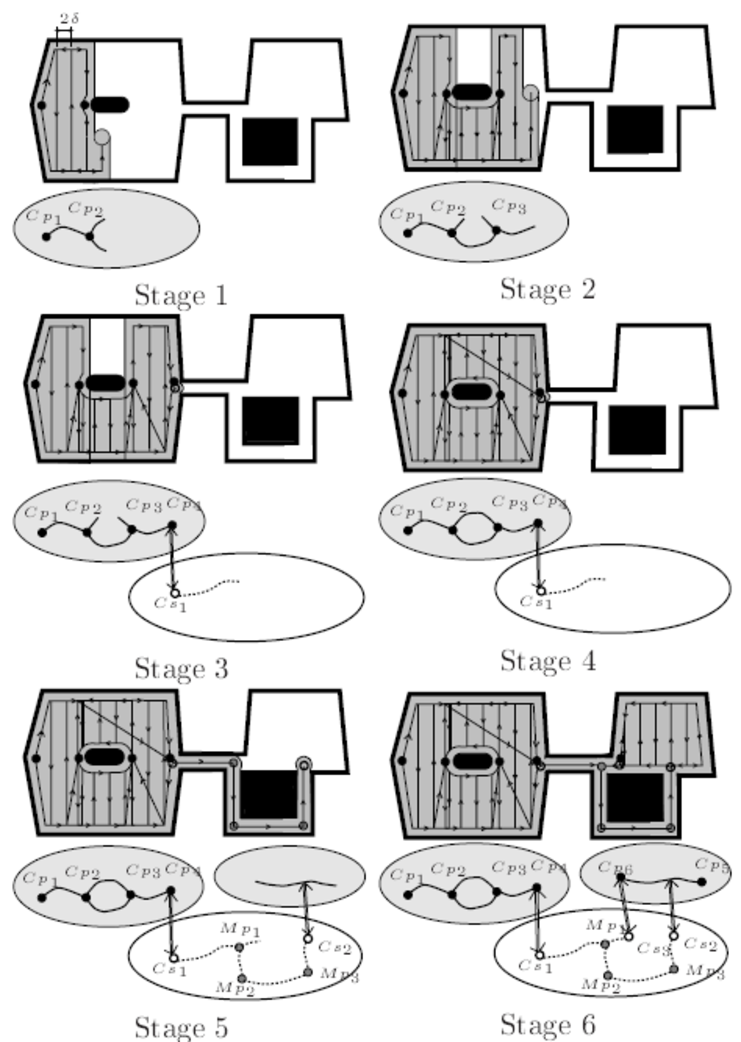
\includegraphics[width=0.5\textwidth,trim=2 2 2 2,clip]{VASTNARROW.pdf}
\end{RoyalFigure}

Figure~\ref{fig:vastnarrow} depicts the stages of the incremental construction of the hierarchical decomposition while
the robot is covering the space. The graphs depicted in the gray ellipses depict the \gls{gls-vast-cell}s that contain
VAST-subcells represented as solid edges. Each VAST-subcell has to associated
\gls{gls-critical-point}s represented as black dots. \gls{gls-narrow-cell}s is represented by the white ellipse and it
contains the NARROW-subcells depicted as dashed edges. Hollow dots correspond to \gls{gls-cusp-point}s
and gray dots represent the meet points. The double arrows show the links between \gls{gls-narrow-cell}s and their
neighboring \gls{gls-vast-cell}s.

\subsection{LANDMARK-BASED TOPOLOGICAL COVERAGE}
The above described Morse-based algorithms create cell boundaries based on the detection of \gls{gls-critical-point}s,
these points are detected via side faced range sensors, with the use of wall following. Morse-based algorithms cannot
handle rectilinear environments, due to the fact that \gls{gls-critical-point}s are degenerate in this environment.
Landmark-based topological coverage algorithm also use the \gls{acr-BCD}, but cell boundaries are determined by using
topological landmarks.

Topological maps are robust against sensor and odometry errors because only a global topological consistency, rather
than a metric one, needs to be maintained. \citet{thrun_learning_1998} states that this type of map does not require
accurate determination of the robot's position. Although this low resolution is also the reason why it's difficult to
use them for \gls{gls-coverage-path} planning. A node in a topological map is a landmark and does not correspond to a
precise position or area in space. This makes it difficult to mark covered regions \cite{wong_qualitative_2006}.

\subsubsection{SLICE DECOMPOSITION}\label{subsec:slicedecomp}
Slice decomposition makes use of simpler landmarks. \citet{galceran_survey_2013} states that it can handle a large
variety of environments including ones with polygonal, elliptical and rectilinear obstacles. Moreover obstacles can be
detected from all sides of the robot, allowing a simpler zig-zag pattern without retracting to be used. As a result the
generated \gls{gls-coverage-path} is shorter.

Slice decomposition determines cell boundaries when it sees a abrupt change in the topology between segments in
consecutive slices, each slice is a sensor sweep line where the \( \gls{sym-delta_s}  x \) is moved to the next time
step. \citeauthor{wong_complete_2004} states that there are two situations where the abrupt changes occurs:

\begin{enumerate}
	\item A segment in the previous slice is split by the emergence of a new segment, see figure~\ref{fig:slicedec} (a) and (b).
	\item A segment from the previous slice disappears in the current slice, see figure~\ref{fig:slicedec} (c) and (d).
\end{enumerate}

\begin{RoyalFigure}[!htb, label=fig:slicedec]{(a) SPLITTING OF SEGMENTS (b) MERGING OF SEGMENTS \cite{wong_complete_2004}}
		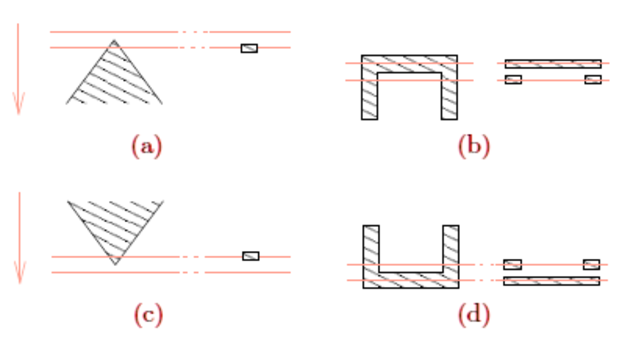
\includegraphics[height=2.5cm,trim=2 2 2 2,clip]{slicedec.pdf}
\end{RoyalFigure}

\begin{RoyalAlgorithm}[label=alg:offlineslicedecomposition]{OFF-LINE SLICE DECOMPOSITION}
	\begin{algorithmic}[1]
		\Procedure{SliceDecomposition}{}
		\State $ \gls{sym-c} \in \{Free Space Cell, Obstacle Cell\} $
		\ForAll{$ \text{time } \gls{sym-t} $}
		\State $ \text{Move sweep line downwards by} \gls{sym-Delta_x}   $
		\State $ \gls{sym-D_l_t-1} = (\ldots, \gls{sym-c}_{i-2}, \gls{sym-c}_{i-1}, \gls{sym-c}_{i}, \gls{sym-c}_{i+1}, \gls{sym-c}_{i+2}, \ldots)$
		\ForAll{$ \text{segments in } \gls{sym-D_l_t-1} $}
		\If{$ \text{emergence inside } \gls{sym-c}_i $}
		\State $(\gls{sym-c}_i) \gets (\gls{sym-c}_{e-1},\gls{sym-c}_{e},\gls{sym-c}_{e+1})$
		\State $ \gls{sym-D_l_t} = (\ldots, \gls{sym-c}_{i-2}, \gls{sym-c}_{i-1}, \gls{sym-c}_{e-1}, \gls{sym-c}_{e}, \gls{sym-c}_{e+1}, \gls{sym-c}_{i+1}, \gls{sym-c}_{i+2}, \ldots) $
		\EndIf
		\If{$ \gls{sym-c}_i \text{disappears} $}
		\State $ (\gls{sym-c}_{i-1}, \gls{sym-c}_i, \gls{sym-c}_{i+1}) \gets (\gls{sym-c}_d) $
		\State $ \gls{sym-D_l_t} = (\dots, \gls{sym-c}_{i-2}, \gls{sym-c}_d, \gls{sym-c}_{i+2}, \dots) $
		\EndIf
		\EndFor
		\EndFor
		\EndProcedure
	\end{algorithmic}
\end{RoyalAlgorithm}

The slice decomposition is a formed by maintaining a list \gls{sym-D_l}, which consist of active obstacles and free
space cells. This list is created via algorithm~\ref{alg:offlineslicedecomposition}. This algorithm consist of two
loops. The first one moves the sweep line, while the second one inspects segments and acts if there is a change in
situation. At this time it updates the list \gls{sym-D_l} marking it landmark. This algorithm does not take into account
``\emph{line of sight}''. The author of this paper states that disappearance of segment can only be measured from
hindsight. Thus backtracking will still be an issue.

\begin{RoyalFigure}[!htb, label=fig:slicedecmpD]{SLICE DECOMPOSITION GENERATED BY ALGORITHM~\ref{alg:offlineslicedecomposition}~\cite{wong_complete_2004}}
		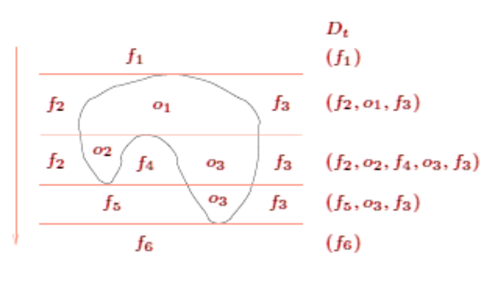
\includegraphics[height=3cm,trim=2 2 2 2,clip]{slicedecompD.pdf}
\end{RoyalFigure}

\citet{wong_qualitative_2006} recognizes the limitations of slice decomposition and proposes a new method ``\emph{slice
decomposition II}''. This is because a robot cannot move inside obstacles, which means that the sweep line is limited to
the cell that the robot is in~\cite{wong_qualitative_2006}. There are five events that occur during slice decomposition
II, as are depicted in figure~\ref{fig:slicedecompII}. \citeauthor{wong_qualitative_2006} proposes the following events
to be used during the \gls{gls-on-line} algorithm~\ref{alg:offlineslicedecompositionII}. If the robot is tethered, for
instance with an \gls{gls-umbilical}, not every cell can be be reached. The restrictions created by this tether can be
view as a change of the boundary of the environment.

\begin{RoyalFigure}[!htb, label=fig:slicedecompII]{(a) SPLIT, (b) MERGE, (c) END, (d) LENGTHEN, (e) SHORTEN}
	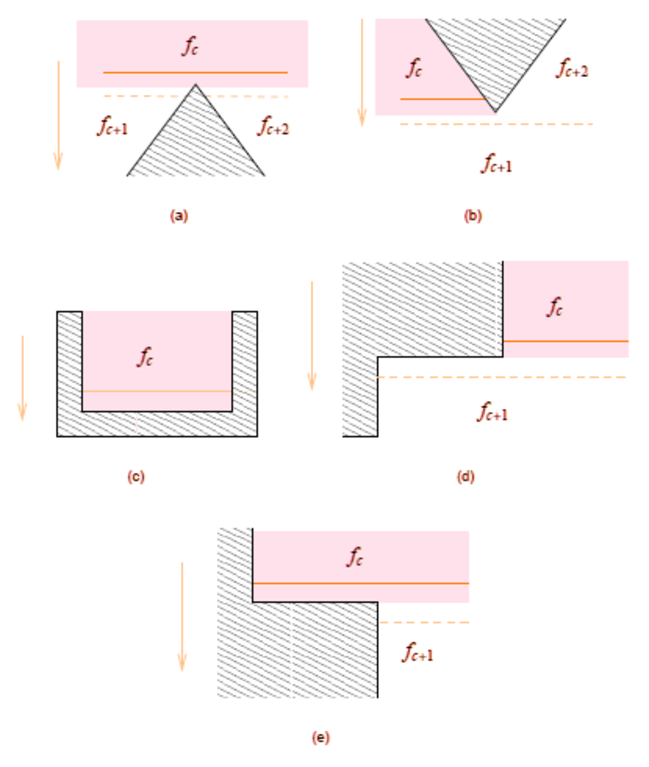
\includegraphics[height=10cm,trim=2 2 2 2,clip]{slicedecompII.pdf}
\end{RoyalFigure}

\begin{RoyalTable}{X[1,l,m] X[4,l,m]}
	\RoyalHeader{ACTION|DESCRIPTION}
	\RoyalRow{SPLIT|Free space segment in the previous slice is split into two by the emergence of an obstacle. This is
	equivalent to obstacle segment emergence in normal Slice Decomposition.}
	\RoyalRow{MERGE|Free space segment in the current slice neighbors free spaces other than the free space segment in the
	previous slice in the direction of the previous slice. This is equivalent to obstacle segment disappearance in normal
	slice decomposition.}
	\RoyalRow{END|The previous free space segment is the final one in the current cell. This is equivalent to free space
	segment disappearance in the normal version.}
	\RoyalRow{LENGTHEN|Free space segment in the current slice neighbors an obstacle segment in addition to the free space
	segment in the previous slice in the direction of the previous slice. Another way to view this situation is that the
	current slice is much longer than the previous slice.}
	\RoyalRow{SHORTEN|Free space segment in the previous slice neighbors and obstacle segment in addition to the free space
	segment in the current slice in the direction of the current slice. Another way to view this situation is that the
	current slice is much shorter than the previous slice.}
\end{RoyalTable}

\begin{RoyalAlgorithm}[label=alg:offlineslicedecompositionII]{OFF-LINE SLICE DECOMPOSITION II}
	\begin{algorithmic}[1]
		\Procedure{SliceDecompositionII}{}
		\State $ O \gets \text{inital cell} $
		\State $ F \gets \emptyset $
		\While{$O \neq  \emptyset$}
			\State $f_c \gets f \in O $
			\State move to on (of two) cell boundary of $ f_c $
			\Repeat
				\State move sweep line by $ \gls{sym-Delta_x}  $ towards the opposite cell boundary
				\If{event occur}
					\State $ F \gets F + f_c $
					\State $ O \gets O - f_c $
					\If{event = split or merge}
						\State $ O \gets O + f_{c+1},f_{c+2} \text{if} f_{c+1},f_{c+2} \notin (O \cup F) $
					\EndIf
					\If{event = lengthen or shorten}
						\State $ O \gets O + f_{c+1} \text{if} f_{c+1} \notin (O \cup F) $
					\EndIf
				\EndIf
			\Until{event occur}
		\EndWhile
		\EndProcedure
	\end{algorithmic}
\end{RoyalAlgorithm}

\subsubsection{ON-LINE TOPOLOGICAL COVERAGE ALGORITHM}
By using slice decomposition II, which is described in Section~\ref{subsec:slicedecomp}, with a topological map. A
crawler can construct it on-line. It now allows in to perform its task in a unknown environment. The topological map
embeds the slice decomposition of an environment by using events as nodes. The map is updated whenever relevant
information becomes available. The path planner  generates a new path un each update, based on the new partial
topological map~\cite{wong_qualitative_2006}.

This topological map is represented as a planar graph, where the nodes represent landmarks (i.e., split, merge, end,
lengthen or shorten, such as depicted in figure~\ref{fig:slicedecompII}) and edges indicate the types of motion required
to travel between nodes they are incident upon. For example, whether the edge is next to a wall and which side the wall
is on. They also store estimated distances separating the two nodes they connect~\cite{galceran_coverage_2012}.

This topological coverage algorithm makes use of a state transition diagram~\ref{dia:statetopo}. In this diagram three
states are described, each with corresponding algorithm (\ref{alg:boundaryStateTopo},~\ref{alg:normalStateTopo}
and~\ref{alg:travelStateTopo}). The crawler is assumed to be placed in a corner near a wall, therefore the boundary state
is considered as entry point.

\begin{RoyalFigure}[!htb, label=dia:statetopo]{STATE TRANSITIONS FOR TOPOLOGICAL COVERAGE ALGORITHM}
	\resizebox{!}{6cm}{
	\begin{tikzpicture}[->,>=stealth',shorten >=1pt,auto,node distance=6cm,
	semithick, every state/.style={minimum size=2cm, align=center}]

	\node[initial,state,fill=RoyalLightGrey]  		(boundary)  		                  	{Boundary\\Algorithm~\ref{alg:boundaryStateTopo}};
	\node[state,fill=RoyalLightGrey]          		(travel)   	[below right of=boundary] 	{Travel\\Algorithm~\ref{alg:travelStateTopo}};
	\node[state,fill=RoyalLightGrey]	  			(normal)   	[right of=boundary] 		{Normal\\Algorithm~\ref{alg:normalStateTopo}};
	\node						(exit)		[right of=normal, xshift=-20mm]	{exit};
	\path (boundary) edge [bend right] node[xshift=-10mm, pos=0.4, align=center, below] {boundary fully\\explored} (travel);
	\path (normal) edge [bend right] node [pos=0.5] {all covered} (exit);
	\path (travel) edge [bend right] node [pos=0.8, align=center, below, xshift=10mm]{arrived at\\uncovered cell} (normal);
	\path (normal) edge [bend right] node [align=center, above] {event occurred\\new landmark reached} (boundary);
	\end{tikzpicture}}
\end{RoyalFigure}

The crawler starts in the \emph{boundary} state by executing algorithm~\ref{alg:boundaryStateTopo}. During this state
the crawler performs a wall following algorithm. When it finds a landmark or it arrives at the end of a strip, it updates
graph \gls{sym-G_adj}. When it's at the end of a strip and the boundary is fully explored it gets in to the state
travel, described in algorithm~\ref{alg:travelStateTopo}, otherwise it turns around and continues in the boundary state.

\begin{RoyalAlgorithm}[label=alg:boundaryStateTopo]{BOUNDARY STATE}
	\begin{algorithmic}[1]
		\Procedure{BoundaryState}{}
		\Loop
		\State move forward along boundary
		\If{at landmark}
		\State update \gls{sym-G_adj}
		\EndIf
		\If{arrive at end of strip}
		\State update \gls{sym-G_adj}
		\If{boundary fully explored}
		\State state $ \Leftarrow $ travel
		\Else
		\State turn around 180\textdegree
		\EndIf
		\EndIf
		\EndLoop
		\EndProcedure
	\end{algorithmic}
\end{RoyalAlgorithm}

Once in the \emph{travel} state, the path is generated that moves the crawler from one cell to another, it does so by
implementing line 5 and 6 from algorithm~\ref{alg:offlineslicedecompositionII} described at
page~\pageref{alg:offlineslicedecompositionII}. Algorithm~\ref{alg:travelStateTopo} is executed in this state. Once it
arrives at an cell its operation state becomes \emph{normal}. A normal boustrophedon zig-zag movement is followed in
this state.

\begin{RoyalAlgorithm}[label=alg:normalStateTopo]{NORMAL STATE}
	\begin{algorithmic}[1]
		\Procedure{NormalState}{}
		\Repeat
			\State follow zigzag pattern
		\Until{at landmark}
		\State update \gls{sym-G_adj}
		\State state $ \Leftarrow $ boundary
		\EndProcedure
	\end{algorithmic}
\end{RoyalAlgorithm}

\begin{RoyalAlgorithm}[label=alg:travelStateTopo]{TRAVEL STATE}
	\begin{algorithmic}[1]
		\Procedure{TravelState}{}
		\State $ T(n) \Leftarrow \text{search } G $
		\If{$ T(n) =\emptyset $}
			\State exit algorithm
		\EndIf
		\While{$ T(n) \neq \emptyset $}
			\State move towards $ T(0) $
			\If{at $ T(0) $}
				$ T(n) \Leftarrow T(n) - { T(0) } $
			\EndIf
		\EndWhile
		\State state $ \Leftarrow $ normal
		\EndProcedure
	\end{algorithmic}
\end{RoyalAlgorithm}

\subsubsection{LANDMARK RECOGNITION USING NEURAL NETWORKS}
\citet{wong_qualitative_2006} proposes a novel idea to classify landmarks using Neural Networks. These are
classification algorithms which approximates the operations of a human brain. \citeauthor{wong_qualitative_2006} build a
test robot with a 360\textdegree rotatable single-beam sonar. Each scan consists of 48 individual sonar-beams taken over
a range of 360\textdegree. This vector is made independent of orientation, by virtually rotating it so that index 0
would always point towards the direction where the sonar range measured the shortest distance, as depicted in
figure~\ref{fig:rotatedsonarvectors}.

\begin{RoyalFigure}[!htb, label=fig:rotatedsonarvectors]{ROTATION OF SONAR READING TO MOST OCCUPIED DIRECTION~\cite{wong_qualitative_2006}}
	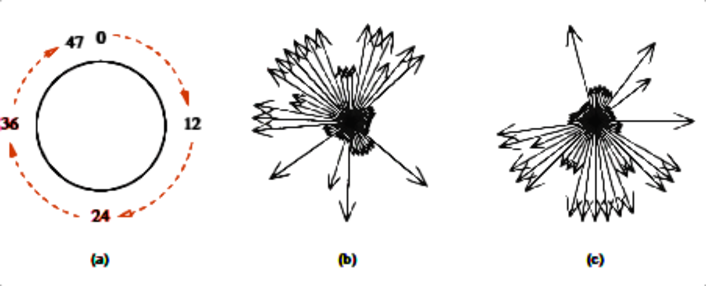
\includegraphics[width=\textwidth,trim=2 2 2 2,clip]{rotatedsonarvectors.pdf}
\end{RoyalFigure}

This vector is fed into a \gls[first]{acr-MLP} which distinguishes three different type of classes: free space nodes,
obstacle nodes and everything else. This neural network first has to be taught. This is done under supervision, meaning
that the landmark type have to be predefined.

\subsection{GRID-BASED METHODS}
Grid-based methods dived the working area into a raster of uniform grid cells. Each cell has an associated value stating
whether an obstacles is present or if it's rather free space. The value can either be binary or a probability
\cite{galceran_coverage_2014}. These grid cells are typically square in shape, but it's not uncommon to use triangle
shaped cell. The size of the cell usually corresponds with the size of a crawler.

\begin{RoyalFigure}[!htb, label=fig:ccpdistancetransform]{COVERAGE PATH GENERATED FROM A DISTANCE TRANSFORM~\cite{wong_qualitative_2006}}
	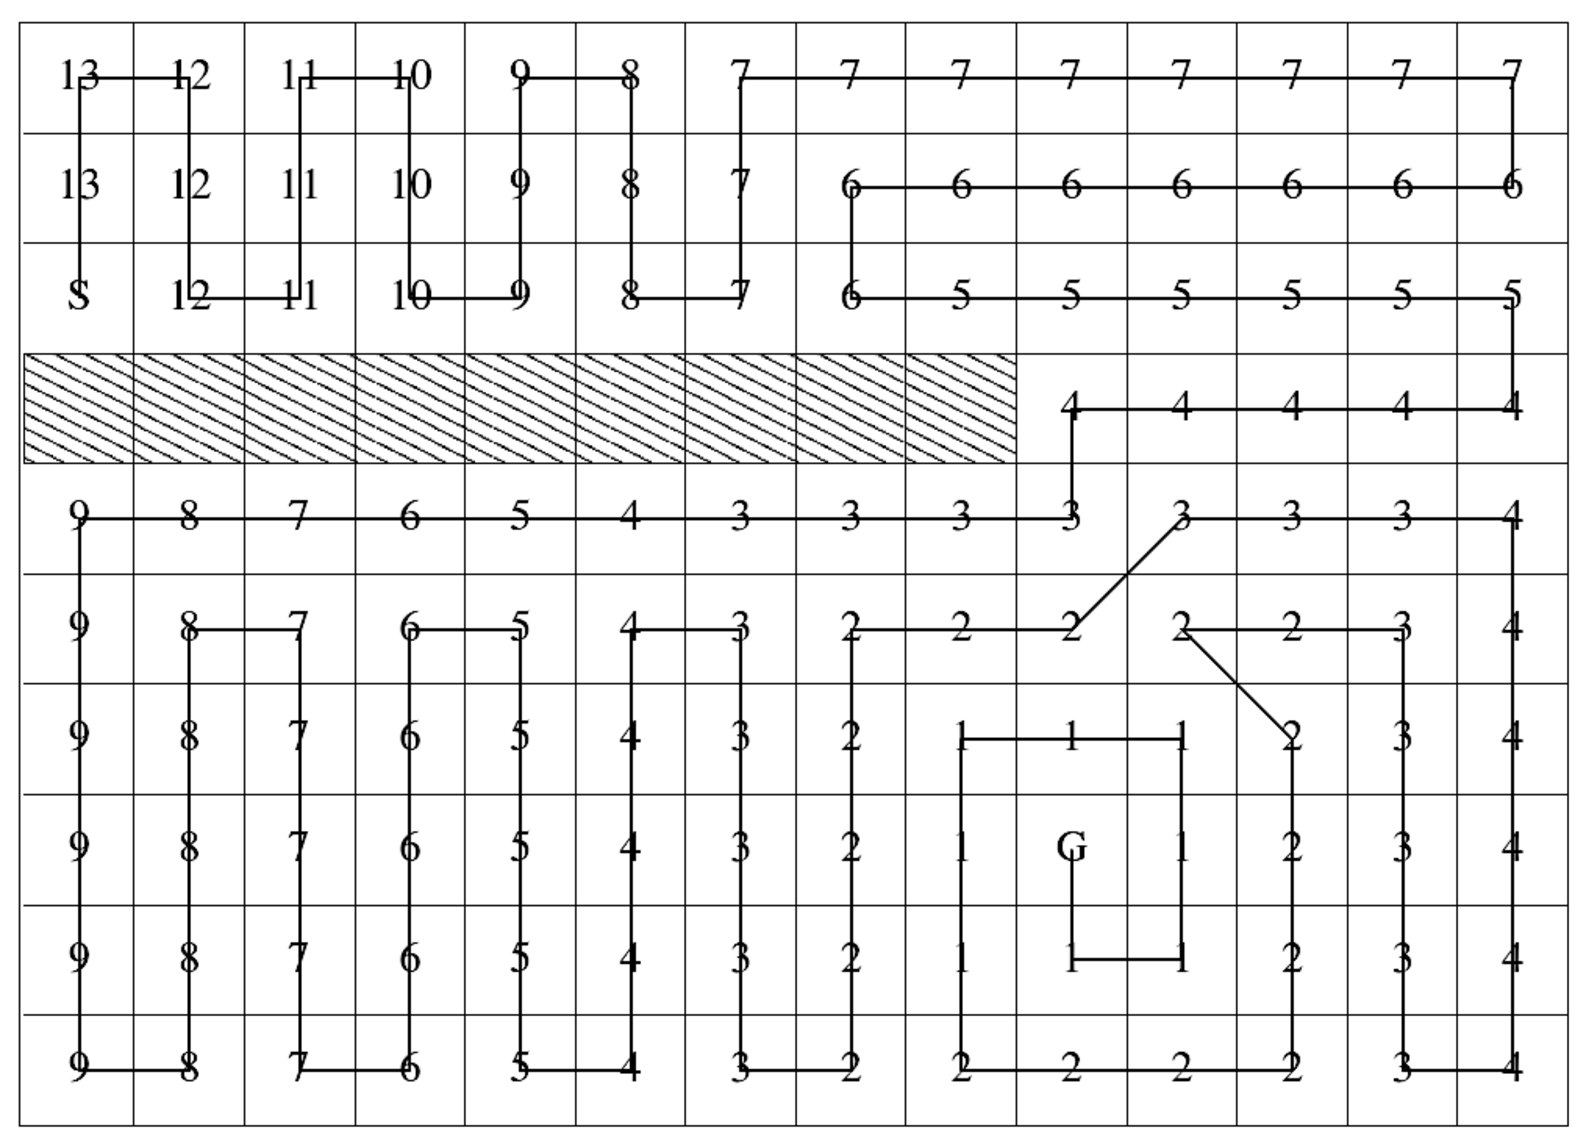
\includegraphics[height=7cm,trim=2 2 2 2,clip]{cppdistancetransform.pdf}
\end{RoyalFigure}

Once the environment is mapped onto an uniform grid. An optimal \gls{gls-coverage-path} can be found using the by
\citet{zelinsky_coverage_1998} proposed method, whom uses a conventional wave-front algorithm (distance transform) to
determine a \gls{gls-coverage-path}. First a start and goal cell has to be assigned. The wave-front algorithm initially
assigns a 0 to the goal and then a 1 to all surrounding [red.~reachable] cells. Then all the unmarked cells neighboring
the marked 1 are then labeled with a 2. This process repeats until the wave-front crosses the start. Once this occurs,
the robot can use gradient descent on this numeric potential function to find a path~\cite{choset_coverage_2001}. This
results of algorithm~\ref{alg:offlinegridbased} is shown in figure~\ref{fig:ccpdistancetransform}.

\begin{RoyalAlgorithm}[label=alg:offlinegridbased]{OFF-LINE GRID-BASED COMPLETE COVERAGE}
	\begin{algorithmic}[1]
		\Procedure{GridBasedCompleteCoverage}{}
		\State Set start cell to current cell
		\State Set all cells to NOT visited
		\Loop
			\State Find unvisited neighboring cell with highest value
			\If{NO unvisited neighboring cell found}
				\State Mark current cell as visited
				\State Exit procedure \Comment{Goal reached}
			\EndIf
			\If{unvisited neighboring cell value $ \leq $ current cell value}
				\State Mark current cell as visited
				\State Exit procdedure \Comment{Goal reached}
			\EndIf
			\State Set current cell to neighboring cell \Comment{Move to next cell}
		\EndLoop
		\EndProcedure
	\end{algorithmic}
\end{RoyalAlgorithm}

The author states an optimal placement of the start and goal cell is paramount. The algorithm~\ref{alg:offlinegridbased}
does not take into account a \gls{gls-deadlock-state}. Which is illustrated in figure~\ref{fig:deadlock}. In this figure
goal and start cell are arbitrarily placed. Execution of the algorithm ensures that the dredge bot is stuck at the
farthest cell. Where it remains, if no backtracking over previous visited cells is allowed.

\begin{RoyalFigure}[!htb, label=fig:deadlock]{DEADLOCK STATE DUE TO INCORRECT STARTING POINT}
		\begin{tikzpicture}[every node/.style={draw,rectangle,minimum size=1cm}]
		\foreach \x in {1,2,3,4,5}
		{
			\foreach \y in {1,2,3,4,5}
			{
				\ifnum\x=1
					\ifnum\y=1
						\node [align=center](\x \y) at (\x,\y) {6\\{\tiny deadlock}};
					\fi
					\ifnum\y=2
						\node [fill=RoyalBlack](\x \y) at (\x,\y) {};
					\fi
					\ifnum\y=3
						\node [](\x \y) at (\x,\y) {4};
					\fi
					\ifnum\y=4
						\node [](\x \y) at (\x,\y) {4};
					\fi
					\ifnum\y=5
						\node [](\x \y) at (\x,\y) {4};
					\fi
				\fi

				\ifnum\x=2
					\ifnum\y=1
						\node [](\x \y) at (\x,\y) {5};
					\fi
					\ifnum\y=2
						\node [fill=RoyalBlack](\x \y) at (\x,\y) {};
					\fi
					\ifnum\y=3
						\node [](\x \y) at (\x,\y) {3};
					\fi
					\ifnum\y=4
						\node [](\x \y) at (\x,\y) {3};
					\fi
					\ifnum\y=5
						\node [](\x \y) at (\x,\y) {3};
					\fi
				\fi

				\ifnum\x=3
					\ifnum\y=1
						\node [](\x \y) at (\x,\y) {4};
					\fi
					\ifnum\y=2
						\node [fill=RoyalBlack](\x \y) at (\x,\y) {};
					\fi
					\ifnum\y=3
						\node [](\x \y) at (\x,\y) {2};
					\fi
					\ifnum\y=4
						\node [](\x \y) at (\x,\y) {S};
					\fi
					\ifnum\y=5
						\node [](\x \y) at (\x,\y) {2};
					\fi
				\fi

				\ifnum\x=4
					\ifnum\y=1
						\node [](\x \y) at (\x,\y) {4};
					\fi
					\ifnum\y=2
						\node [](\x \y) at (\x,\y) {3};
					\fi
					\ifnum\y=3
						\node [](\x \y) at (\x,\y) {2};
					\fi
					\ifnum\y=4
						\node [](\x \y) at (\x,\y) {1};
					\fi
					\ifnum\y=5
						\node [](\x \y) at (\x,\y) {1};
					\fi
				\fi

				\ifnum\x=5
					\ifnum\y=1
						\node [](\x \y) at (\x,\y) {4};
					\fi
					\ifnum\y=2
						\node [](\x \y) at (\x,\y) {3};
					\fi
					\ifnum\y=3
						\node [](\x \y) at (\x,\y) {2};
					\fi
					\ifnum\y=4
						\node [](\x \y) at (\x,\y) {1};
					\fi
					\ifnum\y=5
						\node [](\x \y) at (\x,\y) {G};
					\fi
				\fi

			}
		}

		\draw(34.center) -- (23.center);
		\draw(23.center) -- (13.center);
		\draw(13.center) -- (15.center);
		\draw(15.center) -- (25.center);
		\draw(25.center) -- (24.center);
		\draw(24.center) -- (35.center);
		\draw(35.center) -- (45.center);
		\draw(45.center) -- (44.center);
		\draw(44.center) -- (33.center);
		\draw(33.center) -- (43.center);
		\draw(43.center) -- (41.center);
		\draw(41.center) -- (11.center);
		\end{tikzpicture}
\end{RoyalFigure}

\subsubsection{GRID-BASED COVERAGE USING SPANNING TREES}
An sub-family of grid-based coverage are systematic spiral paths algorithms. These work by following a systematic spiral
spanning tree of a partial grid map. This map is constructed using its on-board sensors~\cite{galceran_coverage_2014}
and uses two different sizes of grid cells. The smaller grid cell is the same size as the robot. Four of these grid
cells then form a mega cell. \cite{wong_qualitative_2006}. The \gls[first]{acr-Spiral-STC} described in
algorithm~\ref{alg:stc}, works as follows:

Starting at the current cell, the robot chooses a new travel direction by selecting the first new mega cell in the free
space in anti-clockwise direction. Then, a new spanning-tree edge is grown from the current mega cell to the new one.
The algorithm is called recursively. The recursion stops only when the current cell has no new neighbors. A mega cell is
considered old if at least one of its four smaller cells is covered. As a result of this recursion, the robot moves
along one side of the spanning tree until it reaches the end of the tree. At this point, the robot turns around to
traverse the other side of the tree~\cite{galceran_coverage_2014}.

\begin{RoyalFigure}[!htb, label=]{COVERAGE PATH GENERATED WITH THE SPIRAL-STC ALGORITHM~\cite{galceran_survey_2013}.}
		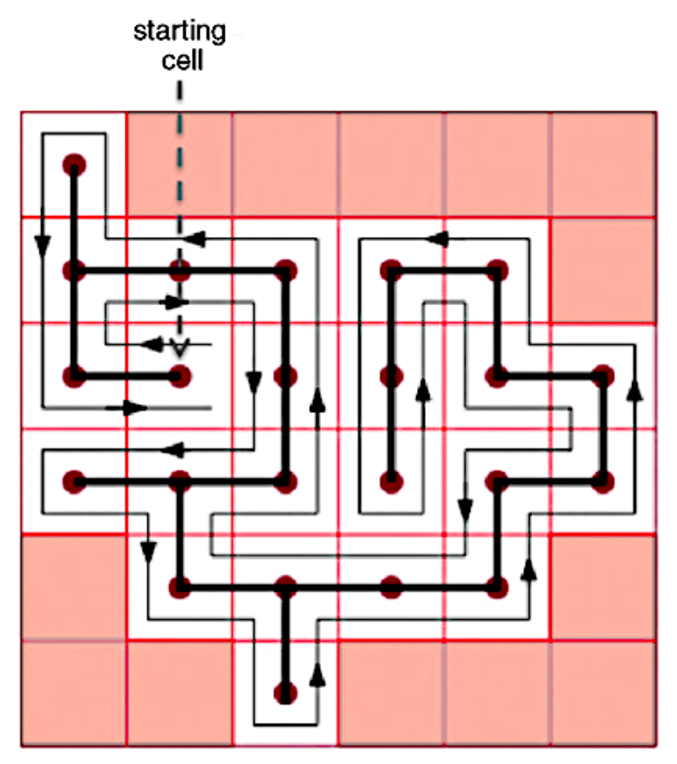
\includegraphics[height=7cm,trim=2 2 2 2,clip]{spiral-stc.pdf}
\end{RoyalFigure}

\begin{RoyalAlgorithm}[label=alg:stc]{SPIRAL SPANNING TREE COVERAGE}
	\begin{algorithmic}[1]
		\Procedure{SpiralSpanningTreeCoverage}{ $ w , \gls{sym-x} $ }
		\State Mark the current cell \gls{sym-x} as $ old $
		\While{\gls{sym-x} has $ new $ obstacle-free-4-neighbour cell }
			\State Scan for the first new neighbour of \gls{sym-x} in anti-clockwise order, starting with the parent cell $ w $ Call this neighbour \gls{sym-y}
			\State Construct a spanning-tree edge from \gls{sym-x} to \gls{sym-y}.
			\State Move to a subcell of \gls{sym-y} by following the right-side of the spanning tree edges
			\State Execute SpiralSpanningTreeCoverage($\gls{sym-x},\gls{sym-y}$).
		\EndWhile
		\If{$ \gls{sym-x} \neq start cell $ }
			\State Move back from \gls{sym-x} to a subcell of $ w $ along the right-side of the spanning tree edges.
		\EndIf
		\EndProcedure
	\end{algorithmic}
\end{RoyalAlgorithm}

\citet{wong_qualitative_2006} and \citet{lee_smooth_2011} states the path can be optimized by using smaller grid cells,
however because accurate maneuverability is often an issue, a higher resolution is not the best approached.
\citeauthor{lee_smooth_2011} proposes a new method for \gls{acr-Spiral-STC} by limiting the number of turns,
decelerations and accelerations. \citet{mei_energy-efficient_2004} determined by analytically comparing energy
efficiency of different coverage algorithm that sharp turns bring about inefficiency. Thus by limiting these, an energy
efficient path can be generated. Since the dredge bot will be powered by an external land-based source, this option
won't be further explored.

\subsubsection{NEURAL NETWORK-BASED COVERAGE ON GRID MAPS}
\citet{luo_solution_2002} proposes a model capable of planning a real-time path; Which covers every area, in
the vicinity of obstacles, to a reasonably extent. A crawlers path is autonomously generated through a dynamic neural
activity landscape~\cite{luo_solution_2002}\cite{luo_bioinspired_2008}. \citeauthor{luo_solution_2002} discretized a 2D
space in a grid map where the diagonal length of each grid cell is equal to the robot sweeping radius and then a neuron
is associated to each and every grid cell. Each neuron has connections to its immediate 8
neighbors~\cite{galceran_survey_2013}. This architecture is illustrated in figure~\ref{fig:cppnn}.

\begin{RoyalFigure}[!htb, label=fig:cppnn]{ARCHITECTURE OF A NEURODYNAMICS MODEL~\cite{yan_complete_2012}}
	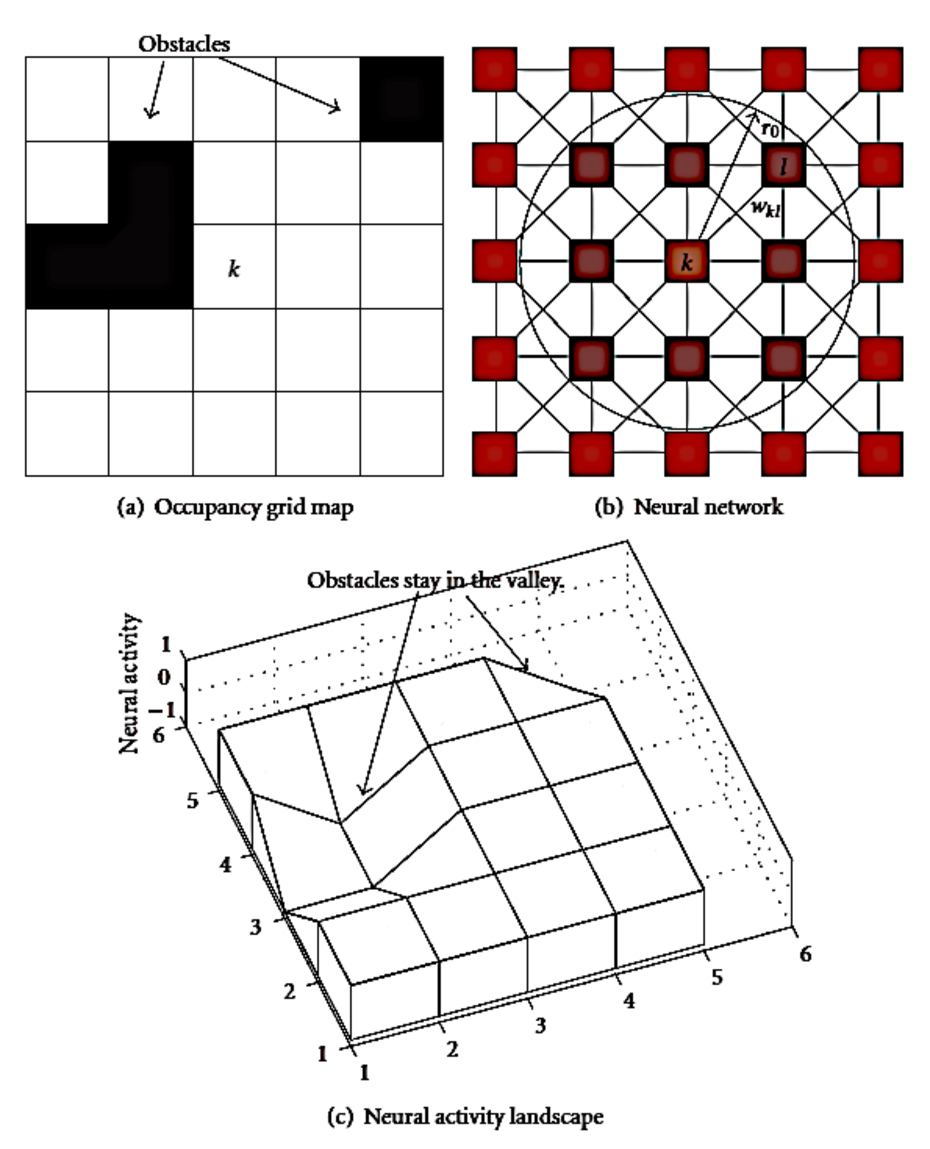
\includegraphics[height=12cm,trim=2 2 2 2,clip]{cppnn.pdf}
\end{RoyalFigure}

The proposed neural network, is topologically expressed on a 2-dimensional occupancy grid map. The location of the
\(k\)th neuron of the neural network represent a location (cell). Where each neuron has local lateral connections
to its neighboring neurons, in the small region \( [0,\gls{sym-r_0}] \); Where \gls[first]{sym-r_0} is the receptive field
radius of the \( k \)th neuron, as shown in figure~\ref{fig:cppnn} (b). The excitatory input results from uncovered area
and lateral neural connections, while inhibitory inputs, results from obstacles~\cite{yan_complete_2012}. The shunting
equation~\ref{eq:shunting} derived from Hodgkin and Huxley~\cite{hodgkin_quantitative_1952} determines the dynamics of
each neuron in the network.

\begin{equation}\label{eq:shunting}
	\dv{x_k}{t} = -Ax_k + (B - x_k) \left(\left[I_k\right]^+ + \sum_{l=1}^{m}w_{kl}\left[\gls{sym-n_a_l}\right]^+ \right) - (D + x_i)\left[I_i\right]^-
\end{equation}

Equation~\ref{eq:shunting} consist of the following terms: \( x_k \) is the \( k \)th neuron in the neural network,
while $A, B \text{ and } D$ are non negative constants describing the passive decay rate, and the upper and lower bounds
of the neural activity. The terms $ \left[I_k\right]^+ + \sum_{l=1}^{m}w_{kl}\left[\gls{sym-n_a_l}\right]^+ $ are the
excitatory inputs while $ \left[I_i\right]^-  $ is the inhibitor. These are linear-above and below thresholds defined as
$ [a]^+ = \max\{a,0\} $ and $ [a]^- = \max\{-a,0\} $. The connection weight is given by $ w_{kl} $ which is assigned
between the $ k $th and the $ l $th neuron, which is given by $ w_{kl} = f(|q_k - q_l|) $, where $ |q_k - q_l| $ is the
Euclidean distance between vectors $ q_k $ and $ q_l $ in the state space, and $ f(d) $is a \gls{gls-monotonically}
decreasing function defined as

\begin{equation}\label{eq:fd}
	f(d) = \left\{
	\begin{array}{ll}
		\frac{\mu}{d}, 0 \leq d < \gls{sym-r_0} \\
		0, d \geq \gls{sym-r_0} \\
	\end{array}
	\right.
\end{equation}

% todo: sym mu
\noindent Where $ \mu $ and $ \gls{sym-r_0} $ are positive constants, The external input $ I_k $ to the $ k $th neuron
is defined in equation~\ref{eq:externalinputs}. In this equation $ E $ is a large constant.

\begin{equation}\label{eq:externalinputs}
	I_k = \left\{
	\begin{array}{ll}
		E, \text{ if it's an uncovered area} \\
		-E, \text{ if it's an obstacle area} \\
		0, \text{ if it's a covered area}\\
	\end{array}
	\right.
\end{equation}

By properly defining the external inputs from the changing environment and internal neural connections, the unclean
areas and obstacles are guaranteed to stay at the peak and the valley of the activity landscape of the neural network,
respectively. The unclean areas globally attract the robot in the whole workspace through neural activity propagation,
while the obstacles have only local effect in a small region to avoid collisions. The collision-free robot motion is
planned in real time based on the dynamic activity landscape of the neural network and the previous robot position, such
that all areas will be cleaned and the robot will travel along a smooth zigzag path~\cite{luo_bioinspired_2008}. An
advantage of this method is that can handle non stationary environments (i.e., dynamically changing obstacles)~
\cite{galceran_survey_2013}.

\citeauthor{yan_complete_2012} further states that if there are power and time limitations, the crawler should
travel the path with the least revisited areas and the least turns of moving directions. Therefore, for a given current
crawler location at time \( k \), denoted by \gls{sym-p_k}, the next crawler location at time \(k + 1\),
\gls{sym-p_k_1} is obtained by equation~\ref{eq:nextauvloc}. Where \( c \) is a positive constant and \gls{sym-m_n} is
the number of neighbouring neurons of the \gls{sym-p_k} neuron, that is all the possible locations of the current
location \gls{sym-p_k}; variable \gls{sym-n_a_l} is the neural activity of the \( l \)th neuron, which is the same as in
equation~\ref{eq:shunting}; \gls{sym-y_l} is a \gls{gls-monotonically} increasing function of the difference  between
the next crawler moving directions, defined in equation~\ref{eq:movementfucntion}.

\begin{equation}\label{eq:nextauvloc}
	\gls{sym-p_k_1} \Longleftarrow x_{\gls{sym-p_k}} = \max\{\gls{sym-n_a_l} + c~\gls{sym-y_l}, l=1,2...,m\}
\end{equation}

Where \( \Delta \varPsi_l \in [0,\pi] \) is the turning angle between the current moving direction and the next moving
direction. Here \( \Delta \varPsi_l = 0 \) is straight ahead, while \( \Delta \varPsi_l  = \pi \) stands for a backwards
movement~\cite{yan_complete_2012}. This would indicated that the crawler only has the ability to turn either left or right
depending on the convention place on  \( \Delta \varPsi_l \). By defining it as \( \Delta \varPsi_l \in [-\pi,\pi] \), the
crawler has a full turning range. Thus \( \Delta \varPsi_l = \varPsi_l - \varPsi_c = |a \tan 2(y_{p_l} - y_{p_c},
x_{p_l} - x_{p_c}) - a \tan 2(y_{p_c} - y_{p_p}, x_{p_c} - x_{p_p})| \)

\begin{equation}\label{eq:movementfucntion}
	y_l = 1 - \frac{\Delta \varPsi_l}{\pi}
\end{equation}

According to \citet{yan_complete_2012} path planning in the vicinity of some unstructured obstacles may cause overlap,
resulting in additional turns, which translates in a higher energy consumption and additional time
\cite{lee_smooth_2011}\cite{algabri_comparative_2015}\cite{mei_energy-efficient_2004}. They propose the use of four
predefined tables as shown in figure~\ref{fig:fourtemp}. These predefined templates are effective to deal with the
vicinity situation of unstructured obstacles and enable the crawler to plan a more reasonable path with less
overlapping areas.

\begin{figure}
	\begin{center}
		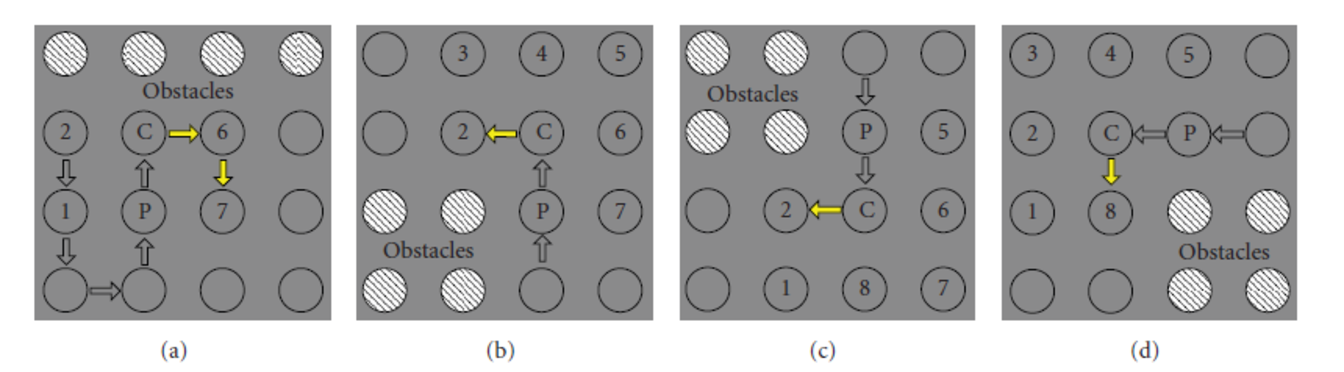
\includegraphics[width=\textwidth,trim=2 2 2 2,clip]{predefinedtemplates.pdf}
	\end{center}
	\caption{Four predefined templates. Source: \citet{yan_complete_2012}}\label{fig:fourtemp}
\end{figure}

Grid based neural networks methods lend themselves to be easily integrated with map building. \citet{yan_complete_2012}
describes how the sensor model can be used to build an on-line map of the environment where the \gls{gls-Dempster-shafer-theory} is used to filter out uncertainties of the sensor.
